% !TEX encoding = UTF-8
% !TEX TS-program = pdflatex
% !TEX root = ../tesi.tex

%**************************************************************
\chapter{Il progetto di stage}
\label{cap:progetto-stage}
%**************************************************************

\section{Analisi dei requisiti}

Ho effettuato l'analisi dei requisiti aiutandomi con quanto fatto durante il progetto precedente, di cui il mio prodotto è un \textit{porting}: le funzionalità offerte dal sistema che ho sviluppato, infatti, devono essere e sono le medesime di tale progetto. Prima di cominciare le attività di progettazione e codifica ho quindi delineato i requisiti richiesti dal progetto al fine di avere uno strumento concreto per verificare l'avanzamento del prodotto e poter validare infine quanto fatto. \\
In questa sezione riporto i casi d'uso dell'applicativo che ho sviluppato; questi non sono parte della documentazione che ho prodotto durante il progetto, ma solo uno strumento a me congeniale per descrivere sinteticamente le funzionalità offerte dal prodotto che ho sviluppato.

\subsection{Casi d'uso}

I casi d'uso consistono in diagrammi che descrivono le possibili interazioni tra l'utente e il sistema. Ogni caso d'uso riportato in questa sezione possiede un codice identificativo, formato nel seguente modo:
\begin{center}
  \centering
  \texttt{UC[codicepadre].[codicefiglio]}
\end{center} dove:
\begin{itemize}
  \item \texttt{UC} significa \texttt{Use Case};
  \item \texttt{[codicepadre]} è un numero progressivo che inizia da 1;
  \item \texttt{[codicefiglio]} è un numero progressivo che inizia da 1 ad ogni incremento di \texttt{[codicepadre]}.
\end{itemize}

Ho qui riportato solamente i casi d'uso principali riguardanti gli attori primari, al fine di esporre chiaramente solo le funzionalità richieste dal sistema oggetto del mio \textit{stage}.

\subsection*{Attori primari}

Gli attori primari, riportati in \hyperref[img:attori]{Figura 3.1}, corrispondono agli utenti che interagiscono con il sistema.

\begin{minipage}{\linewidth}
  \label{img:attori}
  \centering
    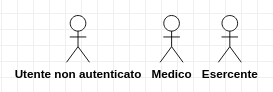
\includegraphics[height=2cm]{immagini/uc/attori}
  \captionof{figure}{Attori principali.}
\end{minipage} \\

Nel sistema del prodotto che ho sviluppato, gli attori principali sono i seguenti:
\begin{itemize}
  \item \textbf{Utente non autenticato}: utente, medico o esercente, che non si è ancora autenticato sulla piattaforma;
  \item \textbf{Medico}: utente che si è autenticato come medico sulla piattaforma;
  \item \textbf{Esercente}: utente che si è autenticato come esercente sulla piattaforma.
\end{itemize}

\subsection*{Diagrammi dei casi d'uso}

\subsubsection*{Utente non autenticato}

La \hyperref[img:nonautenticato]{Figura 3.2} riporta i casi d'uso dell'utente non autenticato.

\begin{minipage}{\linewidth}
  \label{img:nonautenticato}
  \centering
    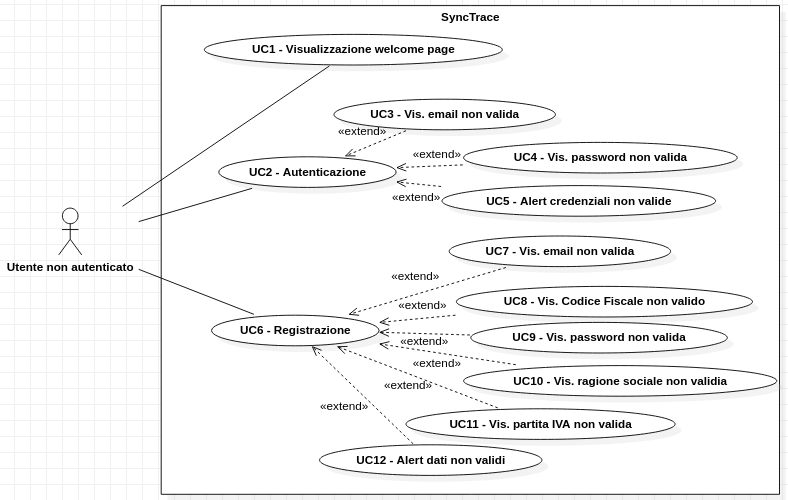
\includegraphics[height=7cm]{immagini/uc/nonautenticato}
  \captionof{figure}{Diagramma dei casi d'uso per un utente non autenticato.}
\end{minipage} \\

\begin{itemize}
  \item \textbf{Attore primario}: l'utente non autenticato;
  \item \textbf{Descrizione}: l'utente non autenticato non può accedere al resto dell'applicazione. Per poterlo fare deve autenticarsi o registrarsi, e questo deve venire offerto dall'applicazione;
  \item \textbf{Precondizione}: l'applicazione offre la possibilità di autenticarsi o registrarsi;
  \item \textbf{Scenario principale}: l'utente non autenticato visualizza la pagina di benvenuto. Dopo aver cliccato sul pulsante \textit{Inizia} può autenticarsi (\texttt{UC2}) o registrarsi (\texttt{UC6});
  \item \textbf{Postcondizione}: l'utente si è autenticato;
  \item \textbf{Estensioni}:
    \begin{itemize}
      \item Se l'utente in autenticazione inserisce una mail o una password mal formattata viene visualizzato un errore sul campo errato (\texttt{UC3} e \texttt{UC4});
      \item Se l'utente tenta di autenticarsi con credenziali non valide viene visualizzato un \textit{alert} (\texttt{UC5});
      \item Se l'utente in registrazione inserisce mail, codice fiscale, password, ragione sociale o partita IVA mal formattati viene visualizzato un errore sul campo errato (\texttt{UC7}, \texttt{UC8}, \texttt{UC9}, \texttt{UC10} e \texttt{UC11});
      \item Se l'utente in registrazione inserisce dati non validi viene visualizzato un \textit{alert} (\texttt{UC12}).
    \end{itemize}
\end{itemize}

\subsubsection*{Medico}

La \hyperref[img:medico]{Figura 3.3} riporta i casi d'uso dell'utente medico.

\begin{minipage}{\linewidth}
  \label{img:medico}
  \centering
    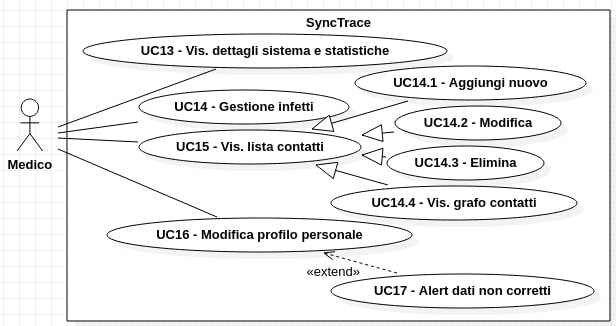
\includegraphics[height=5cm]{immagini/uc/medico}
  \captionof{figure}{Diagramma dei casi d'uso per un utente autenticato come medico.}
\end{minipage} \\

\begin{itemize}
  \item \textbf{Attore primario}: l'utente autenticato come medico;
  \item \textbf{Descrizione}: l'utente medico può accedere alle funzionalità offerte dall'applicazione per il suo ruolo;
  \item \textbf{Precondizione}: l'applicazione permette di accedere alle funzionalità offerte ai medici;
  \item \textbf{Scenario principale}: il medico può visualizzare i dettagli del sistema e le statistiche riguardanti \textit{COVID-19} in Italia (\texttt{UC13}), gestire gli infetti (\texttt{UC14} e sottocasi), visualizzare la lista dei contatti presenti nel sistema (\texttt{UC15}) e modificare il profilo personale (\texttt{UC16});
  \item \textbf{Postcondizione}: l'utente ha utilizzato le funzionalità a lui riservate;
  \item \textbf{Estensioni}: se l'utente modifica i suoi dati inserendo dati errati viene visualizzato un \textit{alert} (\texttt{UC17}).
\end{itemize}

\subsubsection*{Esercente}

La \hyperref[img:esercente]{Figura 3.4} riporta i casi d'uso dell'utente esercente.

\begin{minipage}{\linewidth}
  \label{img:esercente}
  \centering
    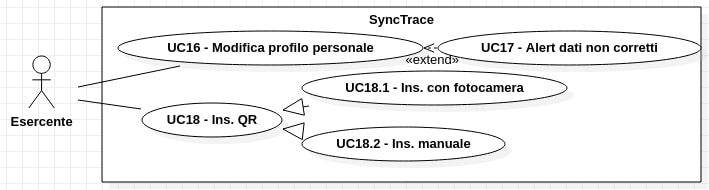
\includegraphics[height=2.5cm]{immagini/uc/esercente}
  \captionof{figure}{Diagramma dei casi d'uso per un utente autenticato come esercente.}
\end{minipage} \\

\begin{itemize}
  \item \textbf{Attore primario}: l'utente autenticato come esercente;
  \item \textbf{Descrizione}: l'utente esercente può accedere alle funzionalità offerte dall'applicazione per il suo ruolo;
  \item \textbf{Precondizione}: l'applicazione permette di accedere alle funzionalità offerte agli esercenti;
  \item \textbf{Scenario principale}: l'esercente può modificare il profilo personale (\texttt{UC16}) e inserire il codice QR (\texttt{UC18}) tramite fotocamera o manualmente (sottocasi di \texttt{UC18});
  \item \textbf{Postcondizione}: l'utente ha utilizzato le funzionalità a lui riservate;
  \item \textbf{Estensioni}: se l'utente modifica i suoi dati inserendo dati errati viene visualizzato un \textit{alert} (\texttt{UC17}).
\end{itemize}

\subsection{Requisiti}

Una volta definiti i casi d'uso ho delineato i requisiti del progetto che sarei andato a sviluppare; per fare ciò sono partito dai requisiti precedentemente definiti e riportati in documentazione, e li ho espansi con i requisiti dell'applicativo oggetto del mio \textit{stage}. Ogni requisito possiede un codice identificativo così definito:
\begin{center}
  \centering
  \texttt{R[tipo][importanza]-[numero]}
\end{center} dove:
\begin{itemize}
  \item \texttt{R} indica che è un requisito;
  \item \texttt{[tipo]} identifica il tipo di requisito. Questo può essere:
  \begin{itemize}
    \item \texttt{F}: requisito funzionale;
    \item \texttt{Q}: requisito qualitativo;
    \item \texttt{V}: requisito di vincolo;
  \end{itemize}
  \item \texttt{[importanza]} identifica l'importanza del requisito. Questa può essere:
  \begin{itemize}
    \item \texttt{O}: requisito obbligatorio;
    \item \texttt{D}: requisito desiderabile;
    \item \texttt{Z}: requisito opzionale;
  \end{itemize}
  \item \texttt{[numero]} identifica il numero del requisito. Esso è composto in tal modo:
  \begin{center}
    \centering
    \texttt{a.b.c}
  \end{center} dove:
  \begin{itemize}
    \item \texttt{a}: numero progressivo che parte da 1 e viene incrementato a ogni nuovo requisito dello stesso tipo e importanza;
    \item \texttt{b}: numero progressivo che parte da 1 e viene incrementato a ogni incremento di \texttt{a};
    \item \texttt{c}: numero progressivo che parte da 1 e viene incrementato a ogni incremento di \texttt{b}.
  \end{itemize}
\end{itemize}

Nell'ambito del precedente \textit{stage} sono stati definiti solo i requisiti funzionali obbligatori riguardanti l'utente non autenticato e l'utente autenticato come medico; a questi ho quindi aggiunto i requisiti funzionali obbligatori riguardanti l'utente autenticato come esercente. \\
Ho inoltre aggiunto altri sei requisiti \textbf{funzionali}, di cui quattro desiderabili e due opzionali, riguardanti l'usabilità dell'applicativo su dispositivi mobili. Per quanto riguarda i requisiti di \textbf{vincolo} ho invece individuato tre requisiti, rifacendomi ai vincoli definiti dal mio \textit{stage}, due dei quali sono individuabili fin da inizio \textit{stage} e riguardano l'utilizzo di determinate tecnologie, e il terzo riguarda l'utilizzo di \textit{Docker} per la containerizzazione del \textit{back-end}, ed è stato quindi aggiunto in corso di sviluppo. Tra i requisiti \textbf{qualitativi}, infine, ho inserito l'utilizzo di analisi statica per la verifica del codice e l'utilizzo di test di unità per la verifica delle funzioni e dei metodi realizzati. \\
Nella \hyperref[tab:totale-requisiti]{Tabella 3.1} riassumo il totale dei requisiti che ho identificato.

\begin{table}[h]
  \label{tab:totale-requisiti}
  \begin{center}
  \begin{tabularx}{\textwidth}{lllll}

                                              & \textbf{Obbligatori}    & \textbf{Desiderabili}  & \textbf{Opzionali}     & \textit{Totale}                  \\ \cline{2-5}
    \multicolumn{1}{l|}{\textbf{Funzionali}}  & \multicolumn{1}{l|}{20} & \multicolumn{1}{l|}{4} & \multicolumn{1}{l|}{2} & \multicolumn{1}{l|}{26}          \\ \cline{2-5}
    \multicolumn{1}{l|}{\textbf{Qualitativi}} & \multicolumn{1}{l|}{2}  & \multicolumn{1}{l|}{0} & \multicolumn{1}{l|}{0} & \multicolumn{1}{l|}{2}           \\ \cline{2-5}
    \multicolumn{1}{l|}{\textbf{Di vincolo}}  & \multicolumn{1}{l|}{3}  & \multicolumn{1}{l|}{0} & \multicolumn{1}{l|}{0} & \multicolumn{1}{l|}{3}           \\ \cline{2-5}
    \multicolumn{1}{l|}{\textit{Totale}}      & \multicolumn{1}{l|}{25} & \multicolumn{1}{l|}{4} & \multicolumn{1}{l|}{2} & \multicolumn{1}{l|}{\textbf{31}} \\ \cline{2-5}
\end{tabularx}
\end{center}
\caption{Totale dei requisiti identificati.}
\end{table}

Considerando che molti dei requisiti funzionali individuati implicano anche numerosi sottorequisiti, il numero totale è certamente importante; nonostante questo, ritengo sia equilibrato rispetto al tempo e alle risorse che ho avuto a disposizione. La ragione di ciò è da ricercarsi nel fatto che 18 di questi requisiti provengono dal precedente progetto: nonostante io abbia dovuto comunque soddisfarli sono infatti stato agevolato nel farlo, non dovendo realizzare da zero le funzionalità ma potendo semplicemente trasporre il codice da una tecnologia a un'altra.

%**************************************************************

\section{Progettazione}

Anche per quanto riguarda le scelte progettuali, essendo il mio progetto la continuazione di un progetto già concluso non ho avuto molto spazio di manovra. Ho però potuto riprogettare l'intera interfaccia grafica dell'applicativo per meglio conformarsi all'utilizzo \textit{mobile} di questo. \\
Prima di procedere alla progettazione vera e propria e alla codifica, ho sviluppato un \textit{mockup} dell'applicazione; poiché le funzionalità offerte dal sistema erano già state definite durante il precedente \textit{stage} su tale progetto, la mia attenzione in questo momento si è rivolta unicamente all'aspetto grafico dell'applicazione che avrei dovuto sviluppare. Per fare ciò ho quindi usato un programma di \textit{sketching}, chiamato \textit{WireframeSketcher}\footcite{tec:wireframesketcher}, per abbozzare l'idea di come avrebbe dovuto essere l'applicazione. Questo programma permette di disegnare \textit{mockup} di siti web e applicazioni \textit{mobile} e \textit{desktop}, mettendo a disposizione numerosi \textit{asset}, quali ad esempio bottoni, campi di testo e \textit{label}, che possono essere facilmente utilizzati per disegnare bozze di applicativi utili ad avere una base di partenza per il successivo sviluppo. \\
Con \textit{WireframeSketcher} ho disegnato le bozze di quasi tutte le maschere che poi ho implementato: ho infatti realizzato 12 maschere, e ho sviluppato la bozza di 10 di queste; questa disuguaglianza trova ragione in una iniziale malinterpretazione dell'applicativo da cui sono partito per lo sviluppo, riguardante le maschere di modifica e visualizzazione degli utenti infetti nel sistema. \\
Non ho riportato questi \textit{mockup} nella documentazione ufficiale fornita come parte del prodotto all'azienda, ma mi sono stati utili per procedere senza indugi nella successiva attività di codifica. Nella \hyperref[img:appsketch]{Figura 3.5} riporto alcuni \textit{sketch} d'esempio. \\

\begin{minipage}{\linewidth}
  \label{img:appsketch}
  \centering
    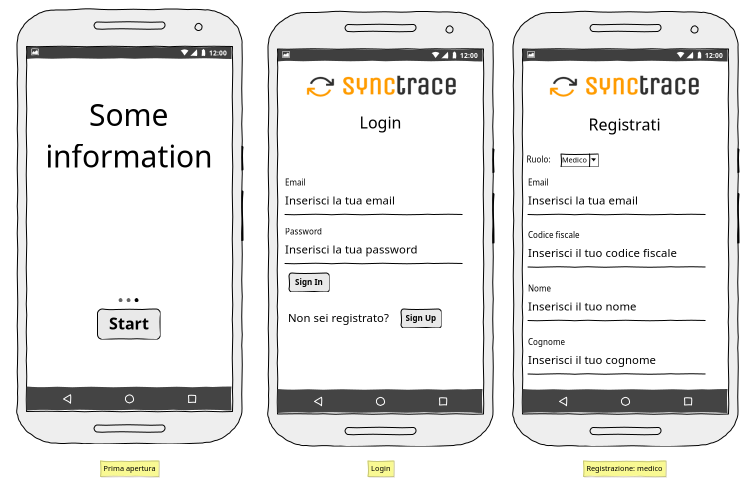
\includegraphics[height=6cm]{immagini/appsketch}
  \captionof{figure}{Esempio di \textit{sketch} dell'applicazione realizzato con \textit{WireframeSketcher}.}
\end{minipage} \\

Come tratterò più approfonditamente nella prossima sezione, sebbene il mio progetto consistesse nella migrazione di una \textit{webapp Angular} su dispositivi mobili è vero anche che il \textit{framework} principale che ho utilizzato è diverso: la \textit{webapp}, infatti, è stata sviluppata totalmente tramite il \textit{framework Angular}, mentre l'applicazione oggetto del mio \textit{stage} è sviluppata tramite il \textit{framework Ionic} che utilizza alcune funzionalità del \textit{framework Angular}, ma è in sostanza una tecnologia diversa. \\
La differenza più evidente tra \textit{Angular} e \textit{Ionic} è che il primo è pensato per lo sviluppo di \textit{single page application}, mentre il secondo è stato creato appositamente per lo sviluppo di applicazioni multipiattaforma, principalmente \textit{mobile}. \textit{Ionic} fa uso del \textit{framework Angular}, del \textit{framework React}\footcite{tec:react} o del \textit{framework Vue}\footcite{tec:vue} per quanto riguarda l'impostazione del progetto, la suddivisione in componenti e la gestione delle \textit{route} tra questi; a questo però aggiunge un sovrastrato per lo sviluppo di una componente \textit{front-end} ottimizzata per dispositivi mobili, \textit{reactive} e \textit{responsive}, composto da numerosi componenti grafici di cui la \hyperref[img:ioniclib]{Figura 3.6} è un esempio. \\

\begin{minipage}{\linewidth}
  \label{img:ioniclib}
  \centering
    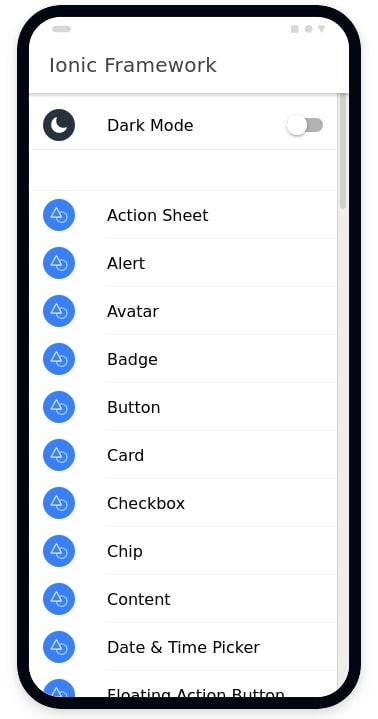
\includegraphics[height=7.5cm]{immagini/ioniclib}
  \captionof{figure}{Esempio di funzionalità proprie di \textit{Ionic}.}
  \caption*{\textbf{Fonte:} ionicframework.com}
\end{minipage} \\

Essendo quindi i \textit{framework} utilizzati per lo sviluppo della \textit{webapp} e dell'applicazione \textit{mobile} differenti, ho dovuto compiere delle scelte progettuali riguardanti la \textbf{sostituzione} di determinati componenti con altri pensati appositamente per l'utilizzo su dispositivi mobili e l'\textbf{aggiunta} del supporto a funzionalità non presenti su dispositivi \textit{desktop}. L'esempio più lampante del primo caso è l'utilizzo della fotocamera: la \textit{webapp}, infatti, fa uso della libreria ZXingScannerModule\footcite{tec:zxingscannermodule}, libreria che non funziona su dispositivi mobili poiché non in grado di richiedere l'autorizzazione all'utilizzo della fotocamera; al suo posto ho utilizzato la libreria qr-scanner di \textit{Ionic Native}\footcite{tec:ionicnative}, che permette di accedere alle componenti hardware richieste. \\
Un esempio di aggiunta di supporto a funzionalità non presenti su dispositivi \textit{desktop} è l'utilizzo di tasti fisici: i dispositivi di input di un computer \textit{desktop} sono infatti principalmente mouse e tastiera, mentre in un dispositivo mobile sono principalmente \textit{touchscreen} e tasti fisici (soprattutto \textit{soft-touch}). Ho quindi dovuto utilizzare il componente backButton della libreria Platform di \textit{Ionic} per garantire il corretto utilizzo del tasto fisico di \textit{back} dei dispositivi mobili. \\
Combinando le attività di analisi dei requisiti e di progettazione ho individuato un totale di quattro importanti componenti da sostituire e sei funzionalità da aggiungere al fine di ottenere un'applicazione \textit{mobile} funzionante, usabile e rasembrante un'applicazione nativa per dispositivi \textit{Android} o \textit{iOS}. A questi si sono poi aggiunti numerosi componenti minoritari di \textit{Ionic} che sono andati a sostituire i rispettivi componenti di \textit{Angular}; esempio di ciò sono i bottoni, i campi dati e le etichette, che su dispositivi \textit{mobile} hanno dicitura e aspetto differenti rispetto a tali componenti implementati su una \textit{webapp Angular}.

%**************************************************************

\section{Codifica}

Una volta conclusa la progettazione sono passato subito all'attività di codifica. Come precedentemente ribadito, il \textit{framework} utilizzato durante il progetto di \textit{stage} precedente al mio e quello che ho invece utilizzato io sono diversi. Un'ulteriore differenza, rispetto a quanto riportato, è che anche gli strumenti a supporto dello sviluppo sono differenti: per la generazione automatica del codice ripetitivo da cui partire con lo sviluppo del codice originale (codice \textit{boilerplate}) con \textit{framework Angular}, infatti, viene utilizzato il \textit{tool AngularCLI}\footcite{tec:angularcli}, mentre con \textit{Ionic} viene utilizzato il \textit{tool IonicCLI}\footcite{tec:ioniccli}. Questo strumento permette la generazione automatica dei componenti, divisi in opportune cartelle come mostra la \hyperref[img:directory]{Figura 3.7}, da cui partire per sviluppare l'applicativo di interesse. In particolare, durante il progetto ho fatto uso di tale strumento per generare i seguenti componenti:
\begin{itemize}
  \item \textbf{Component}: in \textit{Angular}, un \textit{component} è un componente consistente in vista e modello uniti; esso modella quindi sia l'interfaccia grafica che la manipolazione dei dati. In \textit{Ionic}, un \textit{component} è invece concepito come una \textbf{porzione} di applicazione che può essere usata o meno più volte all'interno delle \textit{page}. Un esempio di questo componente in \textit{Ionic} è, nel mio caso, il logo dell'applicazione, che essendo definito come \textit{component} può essere inserito in diverse \textit{page} usando solo la sua dicitura \textit{HTML};
  \item \textbf{Service}: i \textit{service} di \textit{Ionic} coincidono con quelli di \textit{Angular}; essi corrispondono alla \textit{business logic} del progetto, e racchiudono quindi le funzionalità che possono essere utilizzate dagli altri componenti. Nel caso del prodotto sviluppato da me e dagli studenti il cui \textit{stage} ha preceduto il mio, un \textit{service} è ad esempio la componente che si occupa di gestire l'autenticazione degli utenti all'interno del sistema, comunicando con i servizi offerti dal \textit{back-end};
  \item \textbf{Page}: dal punto di vista di \textit{Angular}, una \textit{page} consiste solamente e totalmente in un \textit{component}; in \textit{Ionic}, invece, consiste in un \textit{component} che si comporta come un'intera \textit{view}. Al suo interno, quindi, si possono trovare i \textit{component} precedentemente definiti. Nel mio progetto, ad esempio, una \textit{page} è la maschera di \textit{login}, o una singola maschera visualizzata da un medico o un esercente;
  \item \textbf{Module}: un \textit{module} consiste in un modulo \textit{Angular} che effettua il \textit{bootstrap} in un'applicazione \textit{Ionic}. Lo scopo di tale componente è assicurare che tutti i componenti, le direttive e i \textit{provider} del \textit{framework Ionic} siano importati. Esempi di moduli nel mio progetto sono i \textit{routing module}, che si occupano di gestire le \textit{route} di \textit{Angular} all'interno dell'applicazione.
\end{itemize}
\newpage

\begin{minipage}{\linewidth}
  \label{img:directory}
  \centering
    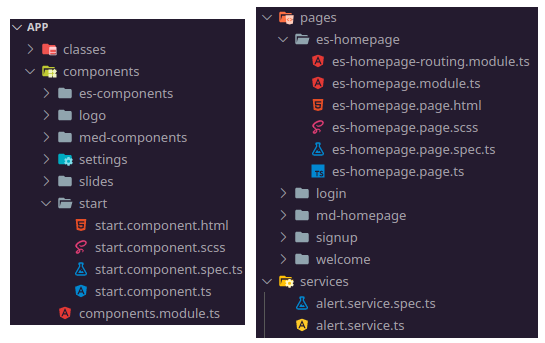
\includegraphics[height=5cm]{immagini/directory}
  \captionof{figure}{Porzioni di \textit{directory} contenente un progetto \textit{Ionic}.}
\end{minipage} \\

Per quanto riguarda lo sviluppo del codice dell'applicazione, ho anzitutto cominciato con le maschere di \textit{login} e \textit{signup}, per permettermi fin da subito di autenticarmi correttamente all'interno del sistema e poter quindi sviluppare le funzionalità previste da entrambi i ruoli. Per la codifica di queste ho fatto un riutilizzo quasi completo dei servizi precedentemente sviluppati, andando a modificare solamente le \textit{route} per permettermi di sviluppare anche la pagina di benvenuto, che viene presentata al primo avvio assoluto dell'applicazione e fintanto che l'utente non si autentica per la prima volta. La \hyperref[img:welcomeloginsignup]{Figura 3.8} mostra queste tre maschere. \\

\begin{minipage}{\linewidth}
  \label{img:welcomeloginsignup}
  \centering
    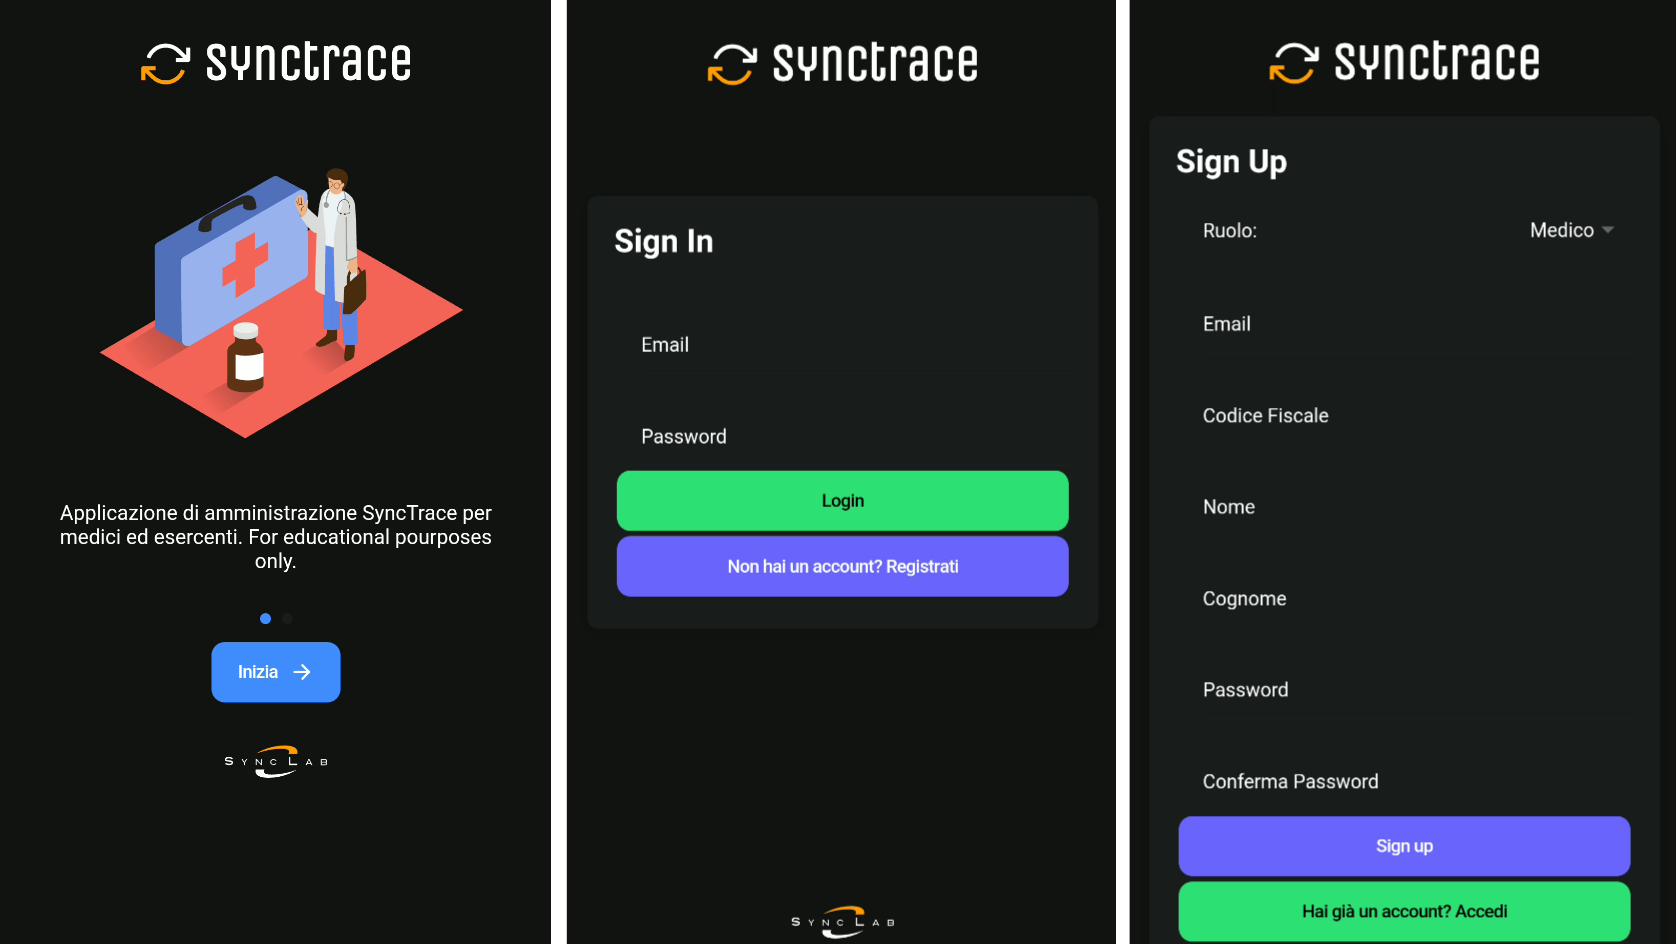
\includegraphics[height=6cm]{immagini/app/welcomeloginsignup}
  \captionof{figure}{In ordine: pagina di benvenuto, \textit{login} e registrazione.}
\end{minipage}\\

Dopo aver realizzato queste prime tre maschere sono passato alla codifica delle maschere riguardanti l'utente con ruolo esercente. Come anticipato precedentemente, l'esercente utilizza l'applicazione per controllare se un cliente può o meno entrare nella sua attività commerciale; per fare ciò, l'esercente legge il codice identificativo del cliente tramite l'applicazione, che comunicherà se questo è o meno infetto o con quale rischio lo è. Per leggere il codice identificativo l'utente ha due possibilità: utilizzare la fotocamera del dispositivo per leggere un codice QR o inserire il codice manualmente. Ho quindi realizzato due maschere, una per modalità di inserimento del codice, come la \hyperref[img:es]{Figura 3.9} riporta.\\

\begin{minipage}{\linewidth}
  \label{img:es}
  \centering
    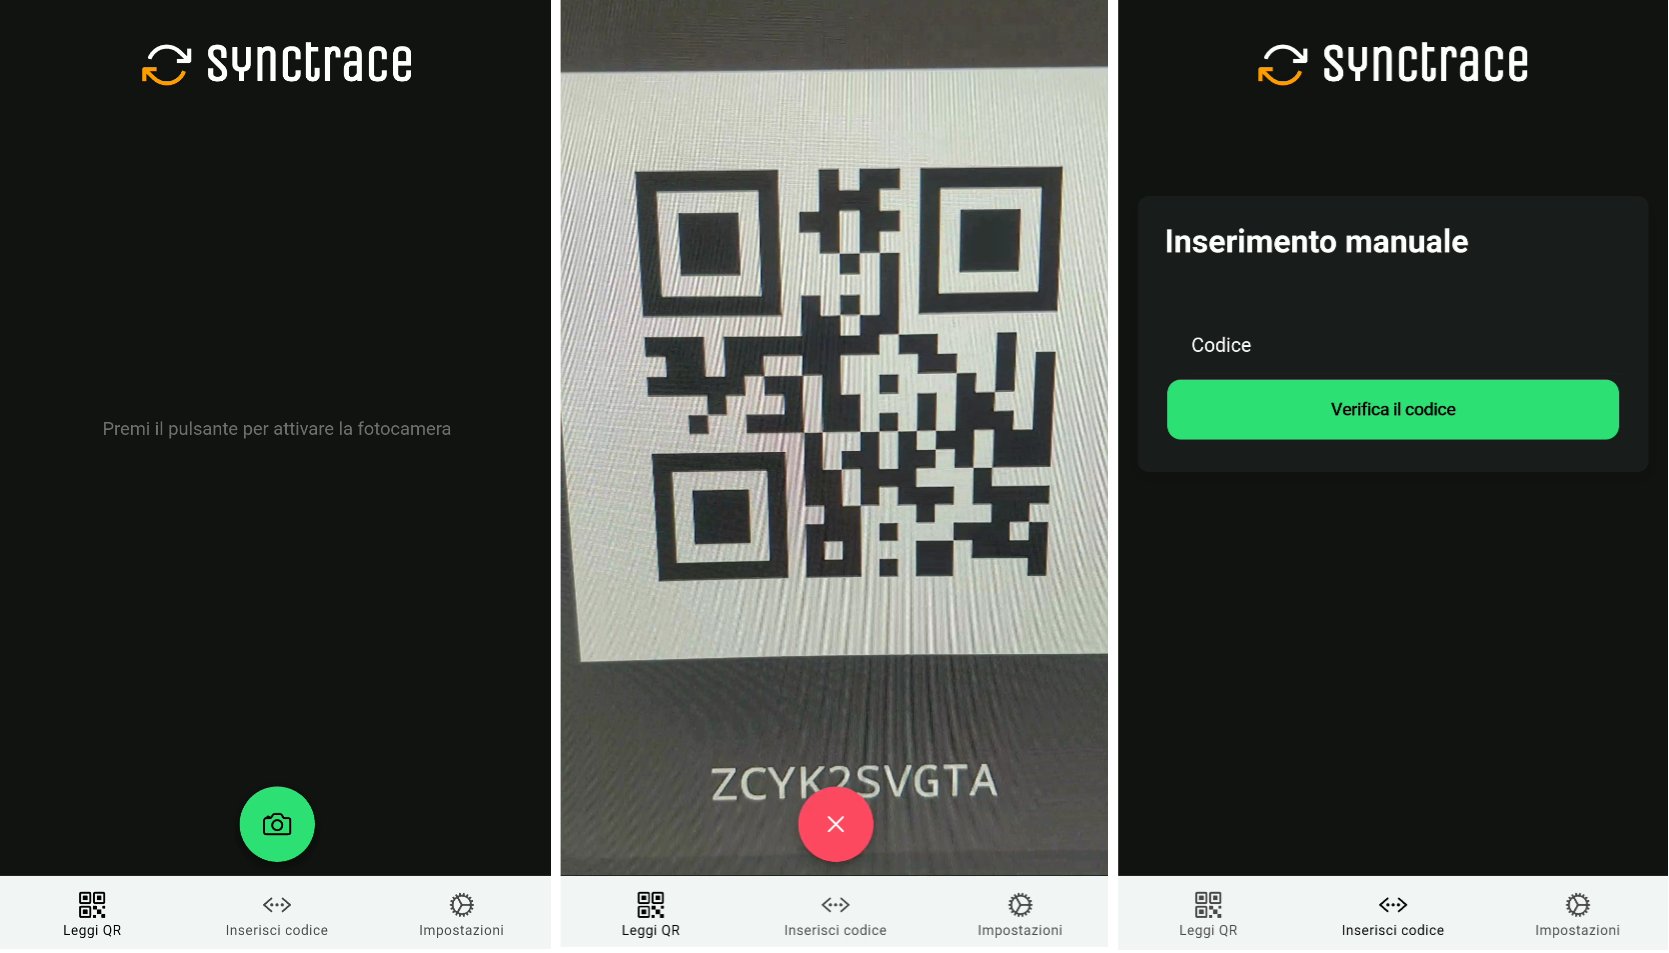
\includegraphics[height=6cm]{immagini/app/es}
  \captionof{figure}{In ordine: lettura del QR a fotocamera spenta, lettura del QR a fotocamera accesa e inserimento manuale.}
\end{minipage}\\

A cavallo tra lo sviluppo delle maschere riguardanti l'esercente e quelle riguardanti il medico, ho codificato la maschera delle impostazioni, raffigurata in \hyperref[img:settings]{Figura 3.10}; da questa vista è possibile visualizzare e modificare le informazioni personali e la password. \\

\begin{minipage}{\linewidth}
  \label{img:settings}
  \centering
    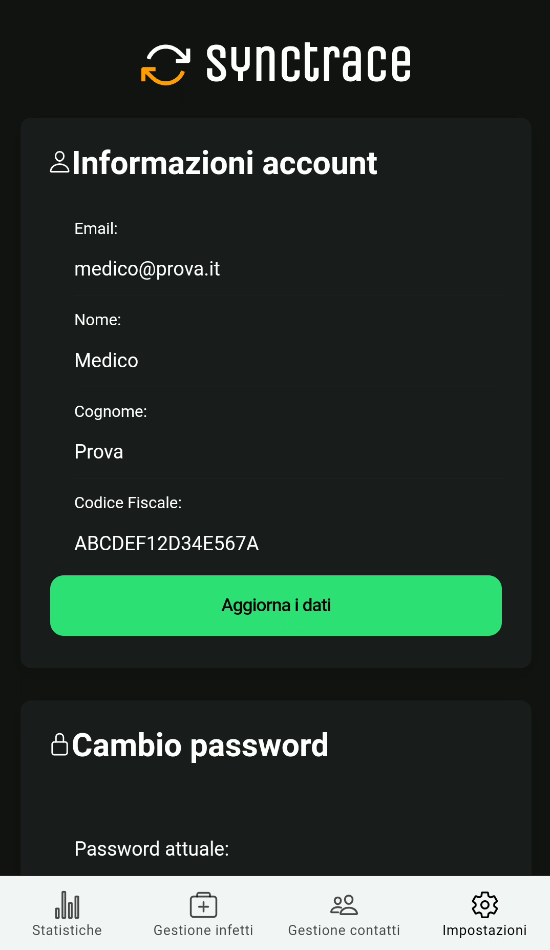
\includegraphics[height=6cm]{immagini/app/settings}
  \captionof{figure}{Maschera delle impostazioni dell'utente.}
\end{minipage}\\

Una volta realizzata questa maschera ho proceduto alla realizzazione delle maschere riguardanti il medico. Come descritto brevemente in precedenza, l'utente medico utilizza l'applicazione per visualizzare le informazioni riguardanti gli infetti e i contatti presenti il tutto il sistema, per gestire gli utenti infetti e visualizzare i contatti tra utenti. Ho quindi realizzato sei maschere per visualizzare i dati, visualizzare, modificare e aggiungere gli utenti infetti e visualizzare i contatti tra gli utenti. Esempi di queste maschere sono quelle che la \hyperref[img:med]{Figura 3.11} rappresenta. \\

\begin{minipage}{\linewidth}
  \label{img:med}
  \centering
    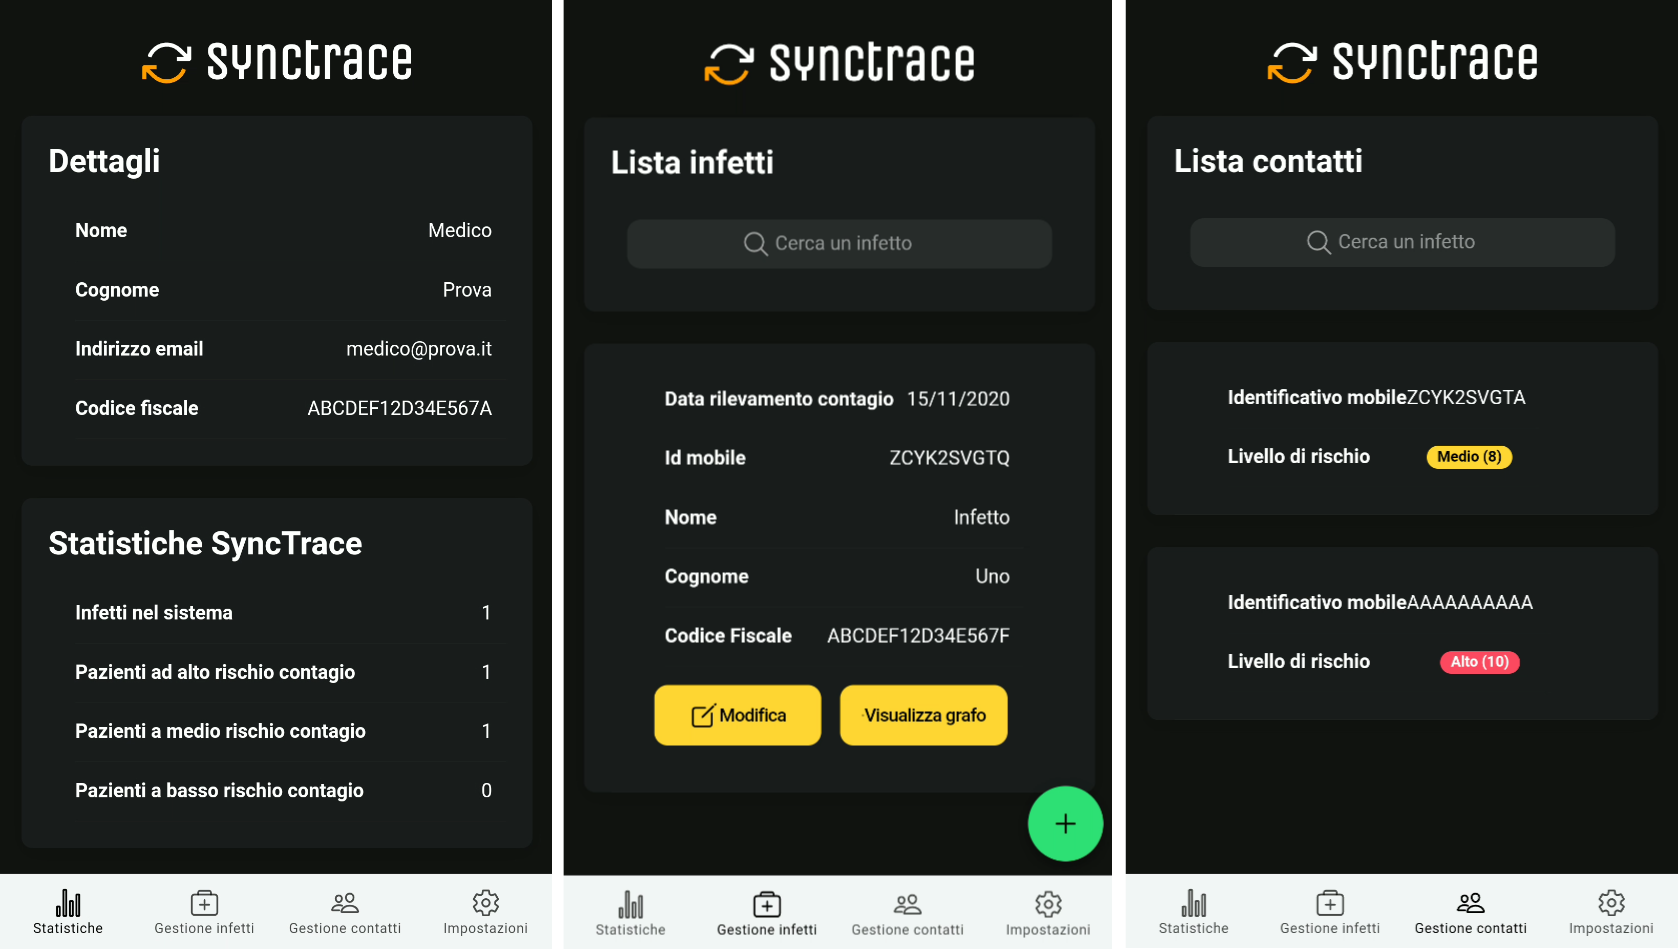
\includegraphics[height=5.5cm]{immagini/app/med}
  \captionof{figure}{In ordine: statistiche del sistema, gestione degli infetti e gestione dei contatti.}
\end{minipage}\\

Durante lo sviluppo delle maschere ho apportato diverse modifiche ai \textit{service} precedentemente sviluppati, al fine di renderli maggiormente compatibili con i dispositivi mobili. In particolare, ho completamente riscritto il servizio di \textit{alert}, poiché quelli nativi del \textit{framework Angular} non sono completamente funzionanti su dispositivi mobili. Al suo posto ho realizzato un servizio che fa uso delle librerie \textit{Ionic Native} per mostrare messaggi di \textit{alert} nativi per dispositivi \textit{Android} e \textit{iOS}. Ho inoltre realizzato un servizio di \textit{toast}, che permette di visualizzare messaggi da parte dell'applicazione sottoforma di \textit{toast}. Entrambi i servizi di avviso sono quindi visualizzati come elementi nativi del sistema operativo mobile, come la \hyperref[img:alert]{Figura 3.12} riporta. \\

\begin{minipage}{\linewidth}
  \label{img:alert}
  \centering
    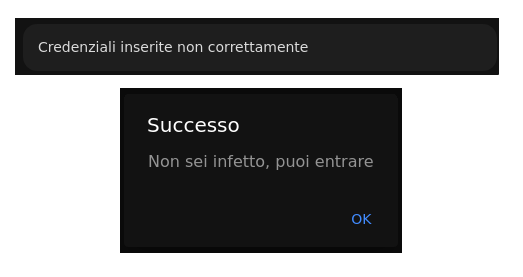
\includegraphics[height=2.7cm]{immagini/app/alert}
  \captionof{figure}{Esempi di, rispettivamente, \textit{toast} e \textit{alert}.}
\end{minipage} \\

Riassumendo, durante l'attività di codifica ho sviluppato 12 maschere, arrivando così a coprire tutti i casi d'uso previsti dal mio \textit{stage} e da quello precedente. Ho inoltre realizzato 8 servizi, 2 dei quali completamente originali e 6 trasposti dall'applicativo \textit{web} di partenza. In \hyperref[tab:sloc]{Tabella 3.2} ho riportato una stima indicativa, precisa nell'ordine delle centinaia, del numero di \textit{SLOC} (\textit{single lines of code}) per ogni linguaggio utilizzato del prodotto che ho sviluppato, indicando anche quante provengono dal progetto precedente al mio (riportate in tabella come \textbf{Iniziali}).

\begin{table}[h]
  \centering
  \label{tab:sloc}
  \begin{tabular}{lll}
    & \textbf{Iniziali}        & \textbf{Finali}                  \\ \cline{2-3}
\multicolumn{1}{l|}{\textbf{TypeScript}} & \multicolumn{1}{l|}{1200} & \multicolumn{1}{l|}{3600}        \\ \cline{2-3}
\multicolumn{1}{l|}{\textbf{HTML}}       & \multicolumn{1}{l|}{0}  & \multicolumn{1}{l|}{700}           \\ \cline{2-3}
\multicolumn{1}{l|}{\textbf{CSS}}        & \multicolumn{1}{l|}{0}  & \multicolumn{1}{l|}{600}           \\ \cline{2-3}
\multicolumn{1}{l|}{\textbf{Commenti}}   & \multicolumn{1}{l|}{0} & \multicolumn{1}{l|}{1200}           \\ \cline{2-3}
\multicolumn{1}{l|}{\textit{Totale}}     & \multicolumn{1}{l|}{1200} & \multicolumn{1}{l|}{\textbf{6100}} \\ \cline{2-3}
\end{tabular}
\caption{Numero indicativo di \textit{SLOC} del prodotto che ho sviluppato.}
\end{table}


%**************************************************************

\section{Verifica}

Sempre a causa del fatto che il mio progetto di \textit{stage} si è basato in gran parte su un prodotto software già completo, ho iniziato il processo di verifica verso la fine dell'attività di codifica: gran parte delle funzioni cruciali, per le quali un \textit{testing} precoce è di indubbia utilità, appartengono infatti ai servizi già precedentemente sviluppati. Ho quindi reputato di scarsa utilità attuare il processo di verifica per la prima parte di sviluppo, poiché in tale periodo mi sono occupato principalmente di codificare in \textit{HTML} e \textit{CSS}; sebbene in questo periodo io abbia creato la maggior parte dei \textit{component} e delle \textit{page}, sviluppate in \textit{TypeScript}, è inoltre vero che il \textit{tool IonicCLI} si occupa di creare i test di unità per il codice automaticamente generato. \\
Quando mi sono avvicinato alla fine dell'attività di codifica ho quindi iniziato il processo di verifica: a questo fine ho svolto due attività, che sono state l'analisi statica e la scrittura di test di unità.


\subsection{Analisi statica}

L'analisi statica è un'attività che prevede la valutazione di un sistema nella sua interezza o di un suo sottoinsieme in base alla sua forma senza la necessità di eseguire il codice. Per quanto riguarda questa attività ho fatto uso principalmente dei metodi \textit{walkthrough} e \textit{inspection}:

\begin{itemize}
  \item \textbf{Walkthrough}: lettura a largo spettro e senza assunzione del codice, mirata a rilevare la presenza di difetti. Ho utilizzato questa tecnica nel momento in cui ho percorso manualmente il codice prodotto simulando possibili esecuzioni;
  \item \textbf{Inspection}: lettura mirata di determinati punti critici del codice. Per utilizzare questa tecnica ho redatto una lista di controllo informale, basata sui punti da me valutati come cruciali anche in seguito all'utilizzo del metodo \textit{walkthrough}.
\end{itemize}

Ho inoltre fatto uso di un \textit{linter}, ossia di un programma di utilità che permette di verificare staticamente il codice in base a parametri predefiniti; nel mio caso ho utilizzato \textit{ESLint}\footcite{tec:eslint}, ossia il \textit{linter} di riferimento per codice \textit{JavaScript} e \textit{TypeScript}. L'utilizzo di questo strumento, correttamente configurato, mi ha permesso di rendere tutto il codice \textit{TypeScript} che ho prodotto aderente agli standard di qualità più stringenti. \textit{ESLint}, inoltre, non si occupa solo della formattazione del codice, ma è anche utile a individuare porzioni di codice duplicato o inutilizzato: ciò mi ha permesso di rilasciare sui \textit{server} di produzione un codice pulito e minimale. \\

\begin{minipage}{\linewidth}
  \label{img:nglint}
  \centering
    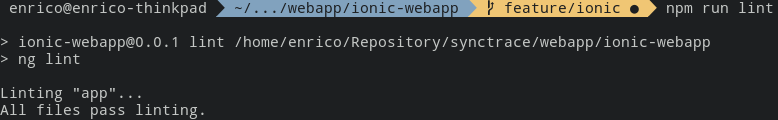
\includegraphics[height=2cm]{immagini/nglint}
  \captionof{figure}{Risultato dell'esecuzione del \textit{linter} sul codice da me prodotto.}
\end{minipage} \\

Ho utilizzato il \textit{linter} per tutti i \textit{file TypeScript} dell'applicazione contenenti logica, compresi i \textit{file} contenenti gli \textit{unit test}, per un totale di 53 \textit{file} esaminati; come mostro in \hyperref[img:nglint]{Figura 3.13}, tutti i \textit{file} analizzati hanno superato i controlli di qualità di \textit{ESLint}.

\subsection{Test di unità}

Parallelamente all'analisi statica ho sviluppato anche dei test di unità; questi sono test che permettono di verificare le singole unità (\textit{i.e.} funzioni, metodi e classi) al fine di determinare se tali unità si comportano nella maniera desiderata. \\
Per realizzare i test di unità ho utilizzato gli strumenti nativi di \textit{Angular}. Questo \textit{framework}, e di conseguenza anche \textit{Ionic}, al momento della generazione di un componente genera anche il codice \textit{boilerplate} per l'implementazione di questi test, di cui la \hyperref[img:jasminetest]{Figura 3.14} è un esempio; nello specifico, per ogni \textit{file} contenente codice \textit{TypeScript} viene generato parallelamente un altro \textit{file TypeScript} con lo stesso nome, a cui viene aggiunto il termine \textit{spec} a indicare che si tratta di un \textit{file} contenente test. \\

\begin{minipage}{\linewidth}
  \label{img:jasminetest}
  \centering
    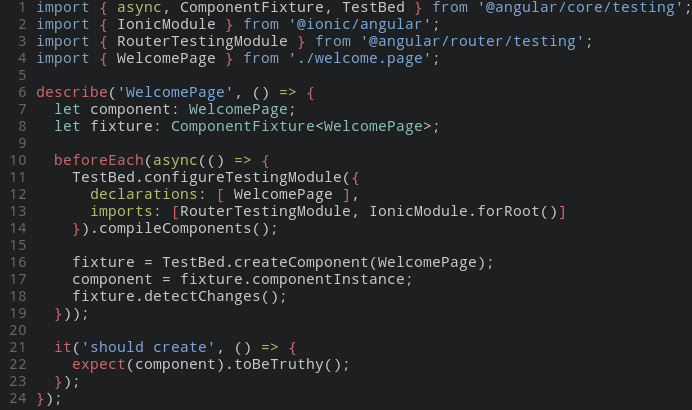
\includegraphics[height=5cm]{immagini/jasminetest}
  \captionof{figure}{Esempio di test di unità \textit{TypeScript}.}
\end{minipage} \\

Lo strumento che si occupa del \textit{testing} in \textit{Angular}, e quindi in \textit{Ionic}, è \textbf{Jasmine}\footcite{tec:jasmine}, un software consistente in un \textit{framework} di test per codice \textit{JavaScript} e \textit{TypeScript}; questo viene eseguito tramite il motore \textit{Karma}\footcite{tec:karma}, che si occupa di eseguire i test e di mostrarli su un \textit{browser} tramite un \textit{server} locale, mostrato in \hyperref[img:jasminekarma]{Figura 3.15}.

\begin{minipage}{\linewidth}
  \label{img:jasminekarma}
  \centering
    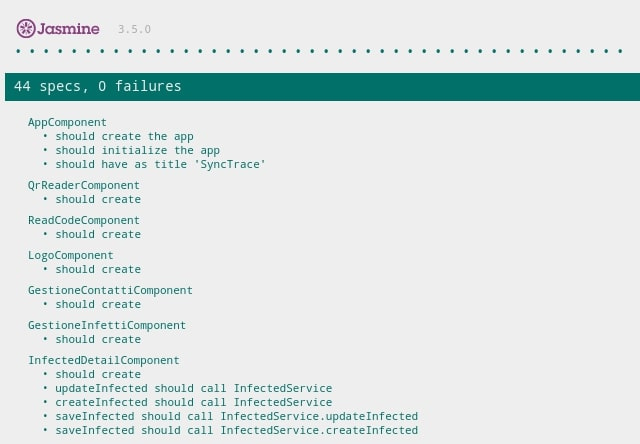
\includegraphics[height=6cm]{immagini/jasminekarma}
  \captionof{figure}{Porzione dell'output di \textit{Jasmine} per il corrente progetto.}
\end{minipage}

In totale ho realizzato 44 test di unità, alcuni dei quali (principalmente delle funzioni riguardanti i \textit{service}) corrispondenti a quelli precedentemente sviluppati.

%**************************************************************

\section{Validazione e collaudo}

Contemporaneamente all'avvio del processo di verifica ho cominciato anche il processo di collaudo, al fine di verificare il funzionamento di tutte le funzionalità anche su dispositivi mobili. Una volta concluso il collaudo sono passato alla validazione, momento in cui ho analizzato insieme al tutor esterno tutti i requisiti che avevo precedentemente definito.

\subsection*{Collaudo}

Come anticipato, parallelamente alla realizzazione dei test di unità e all'analisi statica del codice ho anche collaudato l'applicazione su un dispositivo \textit{mobile}. Vale la pena puntualizzare che non ho effettuato la codifica dell'applicazione a \textit{black-box}, ossia senza controllare periodicamente i risultati di quanto sviluppato; il \textit{framework Ionic}, infatti, possiede una funzionalità di \textit{serve}, che permette la ricarica dinamica dell'applicativo ogniqualvolta venga fatta una modifica al codice. Questo applicativo, però, viene visualizzato in locale nella macchina sul quale sta venendo eseguito lo sviluppo, e più nello specifico viene visualizzato e utilizzato tramite \textit{browser web}, mostrato in \hyperref[img:ionicserve]{Figura 3.16}. Questo è un ottimo strumento di supporto all'attività di codifica, ma non permette di usare l'applicazione su un dispositivo mobile; alcune funzionalità native, infatti, non possono essere utilizzate. \\

\begin{minipage}{\linewidth}
  \label{img:ionicserve}
  \centering
    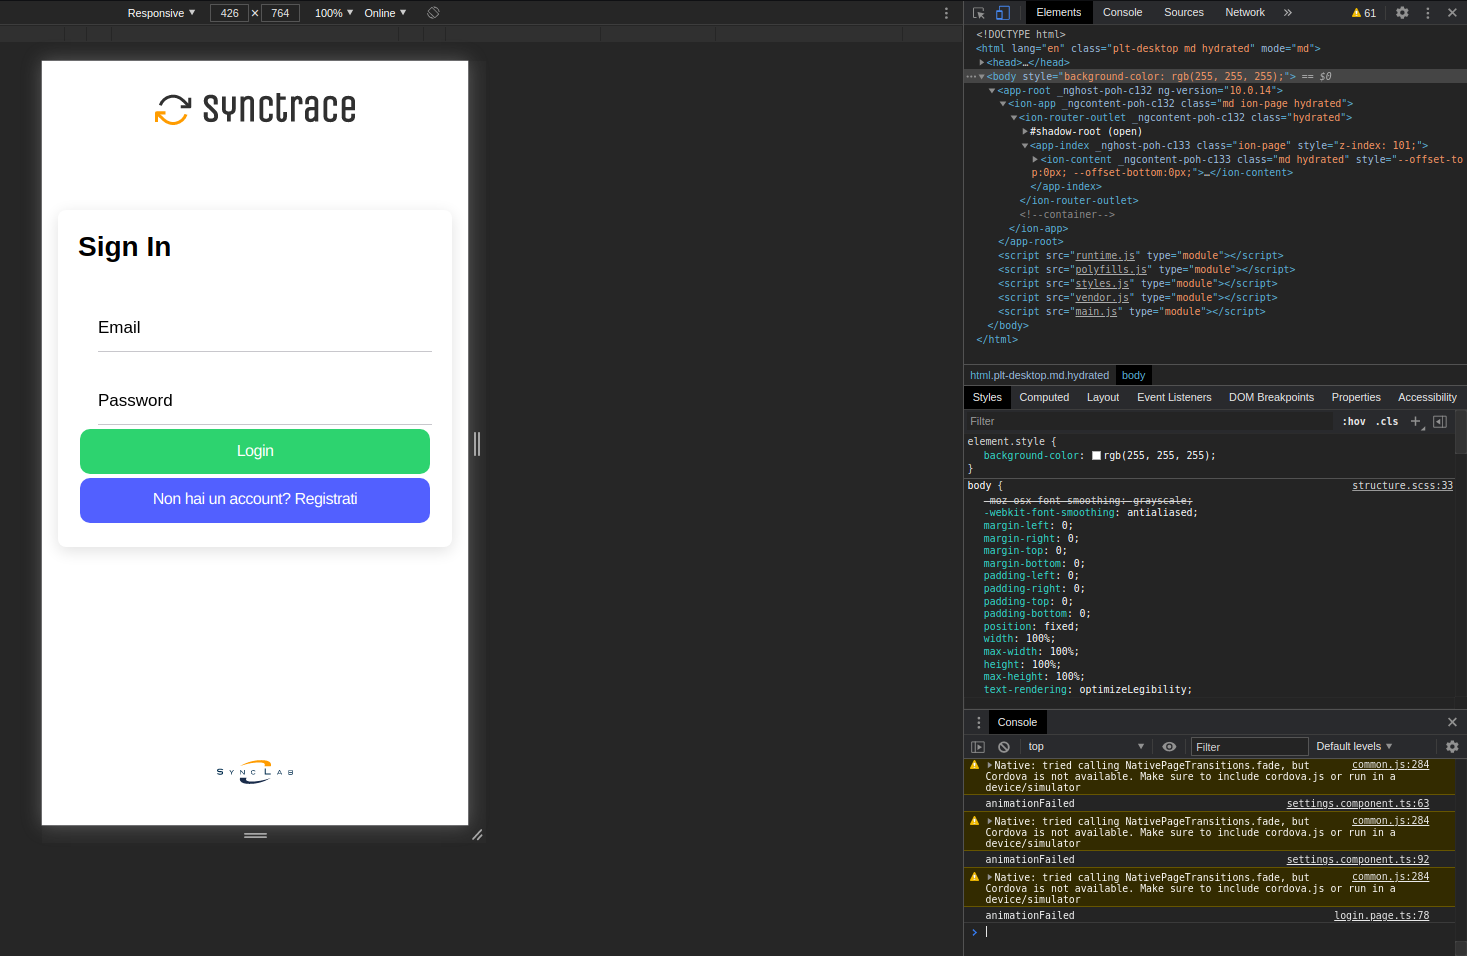
\includegraphics[height=6.8cm]{immagini/ionicserve}
  \captionof{figure}{Esempio di utilizzo di \textit{ionic serve} su \textit{browser Chromium}.}
\end{minipage} \\


Verso la fine dell'attività di codifica ho quindi dovuto poter testare l'applicazione su uno \textit{smartphone}. Nel fare ciò, però, è sorto un problema: fino a quel momento ho eseguito la componente \textit{back-end}, necessaria al funzionamento della maggior parte delle funzionalità dell'applicazione, in locale sulla mia macchina, e questo mi ha reso impossibile il collaudo su un dispositivo mobile. Al fine di poter eseguire questo collaudo, quindi, ho dovuto effettuare il \textit{deployment} del \textit{server} \textit{back-end} su un \textit{server} aziendale. Per fare ciò, mi è stato proposto dal tutor aziendale di containerizzare tale componente tramite la piattaforma \textit{Docker}. Prima di procedere al collaudo, ho quindi interrotto le attività di codifica e verifica per dedicarmi alla trasposizione su \textit{docker machine} del \textit{back-end}. Ho quindi scritto due \textit{file yml}, di cui la \hyperref[img:dockeryml]{Figura 3.17} è un esempio, necessari al comando \textit{docker-compose} di \textit{Docker} per costruire le corrette macchine \textit{docker} e i rispettivi volumi per la persistenza dei dati. \\

\begin{minipage}{\linewidth}
  \label{img:dockeryml}
  \centering
    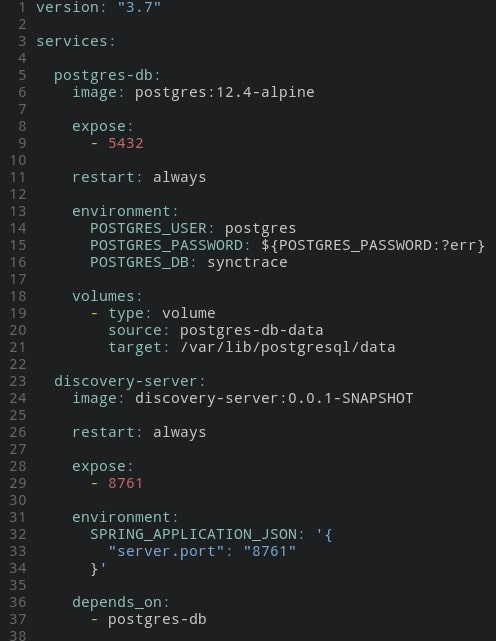
\includegraphics[height=6.4cm]{immagini/dockeryml}
  \captionof{figure}{Porzione del \textit{docker-compose} per i servizi del \textit{back-end}.}
\end{minipage} \\

Una volta effettuato il \textit{deployment} su un \textit{server} aziendale, quindi, sono passato al collaudo vero e proprio dell'applicazione. Ho fatto uso dello strumento \textit{Capacitor}\footcite{tec:capacitor}, ossia un \textit{runtime} che permette la trasposizione di codice \textit{TypeScript} utilizzato all'interno di un progetto \textit{Ionic} in un'applicazione \textit{Android}. Questa applicazione consiste in un \textit{wrapper} che effettua il \textit{render} di una \textit{webview} su dispositivi mobili \textit{Android}, e per l'installazione di questa sul mio dispostivo ho utilizzato \textit{adb} (\textit{Android Debug Bridge}), strumento che mi ha permesso di effettuare anche il \textit{debug} dell'applicazione. \\
Ho quindi redatto una lista di funzionalità di cui controllare il comportamento e l'ho seguita, determinando gli accorgimenti da intraprendere per rendere l'applicazione pienamente funzionante e usabile. Ho infine ripreso l'attività di codifica per correggere gli errori e i malfunzionamenti che sono risultati da questo collaudo.

\subsection*{Validazione}

Alla conclusione delle precedenti attività ho analizzato quanto svolto insieme al tutor esterno, in funzione del soddisfacimento dei requisiti definiti. Il lavoro che ho svolto è stato apprezzabile, poiché ho assolto la maggior parte dei requisiti previsti; nella \hyperref[tab:totale-requisiti-soddifatti]{Tabella 3.3} riassumo i risultati ottenuti.

\begin{table}[h]
  \label{tab:totale-requisiti-soddifatti}
  \begin{center}
    \begin{tabularx}{\textwidth}{lllll}
& \textbf{Totale}         & \textbf{Soddisfatti}    & \textbf{Non soddisfatti} & \textbf{Percentuale}       \\ \cline{2-5}
\multicolumn{1}{l|}{\textbf{Funzionali}}  & \multicolumn{1}{l|}{26} & \multicolumn{1}{l|}{25} & \multicolumn{1}{l|}{1}   & \multicolumn{1}{l|}{96\%}  \\ \cline{2-5}
\multicolumn{1}{l|}{\textbf{Qualitativi}} & \multicolumn{1}{l|}{2}  & \multicolumn{1}{l|}{2}  & \multicolumn{1}{l|}{0}   & \multicolumn{1}{l|}{100\%} \\ \cline{2-5}
\multicolumn{1}{l|}{\textbf{Di vincolo}}  & \multicolumn{1}{l|}{3}  & \multicolumn{1}{l|}{3}  & \multicolumn{1}{l|}{0}   & \multicolumn{1}{l|}{100\%} \\ \cline{2-5}
\end{tabularx}
\end{center}
\caption{Requisiti soddisfatti e non soddisfatti.}
\end{table}

Da questa tabella si può quindi vedere che la maggior parte dei requisiti è stata soddisfatta. L'unico requisito che non ho assolto è il requisito funzionale e opzionale riguardante la \textit{localization}, ossia la traduzione dell'applicazione in lingue diverse da quella italiana; il motivo di ciò è da ricercarsi nella mancanza di tempo che ho avuto all'approssimarsi della fine del mio \textit{stage}.

%**************************************************************

\section{Risultati ottenuti}

Una volta terminato lo sviluppo e validato il prodotto da me creato ho prodotto la documentazione tecnica, al fine di rendere il più possibile esplicite le scelte progettuali che ho effettuato e di rendere trasparente il codice all'azienda e a chi, possibilmente, effettuerà uno \textit{stage} basato sulla porzione di prodotto sviluppata da me. Nel fare questo mi sono affidato allo strumento \textit{Compodoc}; questo software, che si presenta come libreria di \textit{npm}, provvede a creare in automatico la documentazione a partire da commenti strutturati e standardizzati al codice, dei quali la \hyperref[img:compodocdoc]{Figura 3.18} è un esempio.\\

\begin{minipage}{\linewidth}
  \label{img:compodocdoc}
  \centering
    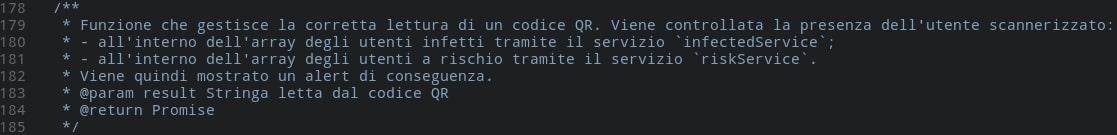
\includegraphics[height=1.5cm]{immagini/compodocdoc}
  \captionof{figure}{Esempio di commento a un metodo per la generazione automatica di documentazione con \textit{Compodoc}.}
\end{minipage} \\

Ho quindi documentato tutte le classi, i parametri, i metodi e le funzioni dell'applicativo, compresi quelli non sviluppati da me, arrivando a raggiungere una \textit{documentation coverage} del \textbf{100\%}. \\

Al concludersi del mio progetto di \textit{stage} ho quindi integrato quanto ho sviluppato nell'intero sistema \textit{SyncTrace}. La somma del mio e degli altri progetti di \textit{stage} ha quindi dato vita a un prodotto completo, che copre i bisogni dettati dal tracciamento dei contatti a tutto tondo, soddisfacendo sia la necessità di tracciare i contatti tra persone che quella di gestire tali dati, nel caso dei medici, e di utilizzarli per mettere in sicurezza la propria attività come nel caso degli esercenti. La porzione di prodotto sviluppato da me, in particolare, semplifica a queste ultime due figure lo svolgimento dei rispettivi ruoli. \\
